\documentclass[11pt]{article}\usepackage[]{graphicx}\usepackage[]{color}
% maxwidth is the original width if it is less than linewidth
% otherwise use linewidth (to make sure the graphics do not exceed the margin)
\makeatletter
\def\maxwidth{ %
  \ifdim\Gin@nat@width>\linewidth
    \linewidth
  \else
    \Gin@nat@width
  \fi
}
\makeatother

\definecolor{fgcolor}{rgb}{0.345, 0.345, 0.345}
\newcommand{\hlnum}[1]{\textcolor[rgb]{0.686,0.059,0.569}{#1}}%
\newcommand{\hlstr}[1]{\textcolor[rgb]{0.192,0.494,0.8}{#1}}%
\newcommand{\hlcom}[1]{\textcolor[rgb]{0.678,0.584,0.686}{\textit{#1}}}%
\newcommand{\hlopt}[1]{\textcolor[rgb]{0,0,0}{#1}}%
\newcommand{\hlstd}[1]{\textcolor[rgb]{0.345,0.345,0.345}{#1}}%
\newcommand{\hlkwa}[1]{\textcolor[rgb]{0.161,0.373,0.58}{\textbf{#1}}}%
\newcommand{\hlkwb}[1]{\textcolor[rgb]{0.69,0.353,0.396}{#1}}%
\newcommand{\hlkwc}[1]{\textcolor[rgb]{0.333,0.667,0.333}{#1}}%
\newcommand{\hlkwd}[1]{\textcolor[rgb]{0.737,0.353,0.396}{\textbf{#1}}}%
\let\hlipl\hlkwb

\usepackage{framed}
\makeatletter
\newenvironment{kframe}{%
 \def\at@end@of@kframe{}%
 \ifinner\ifhmode%
  \def\at@end@of@kframe{\end{minipage}}%
  \begin{minipage}{\columnwidth}%
 \fi\fi%
 \def\FrameCommand##1{\hskip\@totalleftmargin \hskip-\fboxsep
 \colorbox{shadecolor}{##1}\hskip-\fboxsep
     % There is no \\@totalrightmargin, so:
     \hskip-\linewidth \hskip-\@totalleftmargin \hskip\columnwidth}%
 \MakeFramed {\advance\hsize-\width
   \@totalleftmargin\z@ \linewidth\hsize
   \@setminipage}}%
 {\par\unskip\endMakeFramed%
 \at@end@of@kframe}
\makeatother

\definecolor{shadecolor}{rgb}{.97, .97, .97}
\definecolor{messagecolor}{rgb}{0, 0, 0}
\definecolor{warningcolor}{rgb}{1, 0, 1}
\definecolor{errorcolor}{rgb}{1, 0, 0}
\newenvironment{knitrout}{}{} % an empty environment to be redefined in TeX

\usepackage{alltt}
\usepackage{amsmath}
\usepackage{amssymb}
\usepackage{geometry}
\usepackage{graphicx}
\usepackage{fullpage}
\usepackage{enumerate}
\IfFileExists{upquote.sty}{\usepackage{upquote}}{}
\begin{document}
\setlength\parindent{0pt}

Lecture 8: Hypothesis Testing for a Proportion\\
Practice Problems\\
STAT 310, Spring 2021\\

\textbf{Exercise 1}.  It is believed that nearsightedness affects about 8\% of all children.  In a random sample of 194 children, 21 are nearsighted.  Conduct a hypothesis test for the following question: do these data provide evidence that the 8\% value is inaccurate?
% OI 5.32
%400 students were randomly sampled from a large university, and 289 said they did not get enough sleep.  Conduct a hypothesis test to check whether this represents a statistically significant difference from 50\%.
%From \emph{OpenIntro}, fourth edition, Exercise 5.22
\begin{enumerate}[(a)]
\item Write the null and alternative hypothesis for a two-sided test.\\
\vspace{1.5cm}

\item Check the conditions for the hypothesis test.\\
\vspace{1.5cm}

\item Calculate the test statistic.\\
\vspace{2cm}

\item Calculate the $p$-value and make a decision using $\alpha = 0.05$ significance level.\\
\vspace{2.5cm}

\item What is the conclusion of the test in the context of the data?\\
\vspace{2cm}

\item What type of testing error might we have made?
\end{enumerate}
%From \emph{OpenIntro}, fourth edition, Exercise 5.22

\newpage

\textbf{Exercise 2}.  Find the $p$-value for the given $z$-test statistic for a hypothesis test for a proportion.  Also determine if the null hypothesis would be rejected at $\alpha = 0.05$.  Assume all the conditions for the hypothesis test are satisfied.
\begin{enumerate}[(a)]
\item $H_A: p < p_0$; $z = -1.25$\\
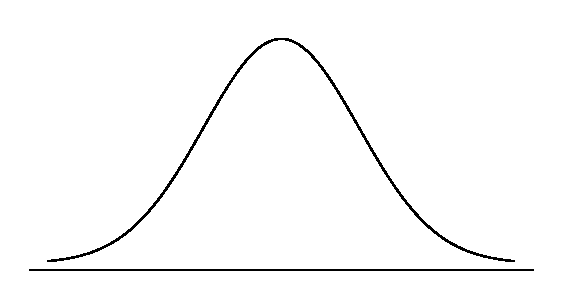
\includegraphics[scale=0.5]{figure/norm_draw}\\
\vspace{2cm}

\item $H_A: p > p_0$; $z = 2.5$\\
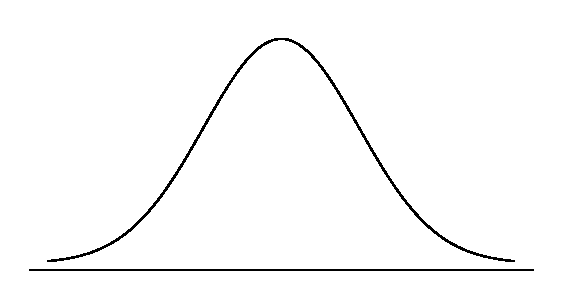
\includegraphics[scale=0.5]{figure/norm_draw}\\
\vspace{2cm}

\item $H_A: p \neq p_0$; $z = -3$\\
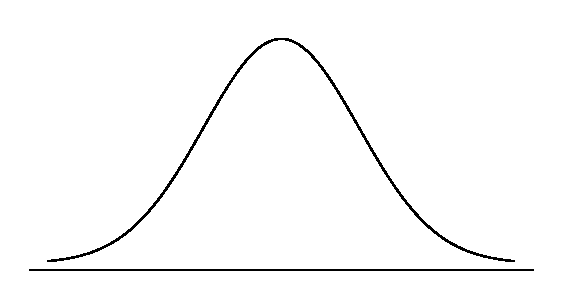
\includegraphics[scale=0.5]{figure/norm_draw}\\
\end{enumerate}





\end{document}
